% Ubah kalimat sesuai dengan judul dari bab ini
\chapter{TINJAUAN PUSTAKA}

% Ubah konten-konten berikut sesuai dengan yang ingin diisi pada bab ini

\section{\textit{Magnetic Imaging Resonance}}

\textit{Magnetic Resonance Imaging} (MRI) adalah teknik pencitraan medis non-invasif yang menghasilkan gambar dengan resolusi tinggi dan kontras jaringan lunak yang sangat baik, memungkinkan visualisasi struktur internal tubuh secara detail dalam format tiga dimensi. Dalam lima tahun terakhir, perkembangan signifikan terjadi pada sistem \textit{low-field} MRI yang kini mampu memberikan performa klinis mendekati \textit{high-field} MRI, dengan keunggulan seperti biaya lebih rendah dan keamanan yang lebih baik untuk pasien tertentu \citep{Hori2021,Huo2025}. Selain itu, real-time MRI (RT-MRI) memungkinkan pencitraan proses dinamis secara langsung tanpa perlu pengulangan, sangat berguna untuk organ yang bergerak seperti jantung dan saluran pencernaan, serta dalam panduan prosedur intervensional \citep{Nayak2022}. Dengan kemajuan teknologi ini, MRI menjadi alat diagnostik yang esensial dalam berbagai bidang medis, termasuk neurologi, kardiologi, dan onkologi, dengan kemampuan yang terus ditingkatkan untuk menghasilkan citra berkualitas tinggi dan informasi fungsional yang mendalam \citep{Hori2021,Nayak2022,Thomas2023}

\section{Artefak MRI}

Artefak dalam pencitraan MRI merupakan masalah yang timbul karena akuisisi citra yang lambat dan sekuensial, dimana data dikumpulkan pada k-ruang (\textit{k-space}) \citep{Liu2020}. Dalam pencitraan otak, artefak gerak (\textit{motion artifacts}) adalah jenis degradasi citra yang paling sering ditemui \citep{Sommer2020}. Artefak ini timbul dari gerakan pasien, baik secara sengaja maupun tidak disengaja karena proses yang dibutuhkan untuk mengumpulkan data citra cukup lama \citep{Al-masni2022}. Artefak gerakan biasanya tampak sebagai \textit{blur} atau bayangan (\textit{ghosting}) pada \textit{phase encoding direction}, yang dapat menurunkan kualitas citra hingga tidak dapat digunakan untuk diagnosis \citep{Liu2020}. Bahkan, artefak gerakan dapat memengaruhi 10\% hingga 42\% pemeriksaan MRI otak, dan dapat menimbulkan bias sistematis dalam perkiraan morfometrik struktur otak \citep{Sommer2020, Vakli2023}.

\section{\textit{ResNet}}

ResNet (\textit{Residual Network}) adalah arsitektur \textit{deep neural network} yang dirancang untuk mengatasi masalah degradasi performa pada \textit{deep network} dengan menggunakan mekanisme \textit{residual learning} melalui \textit{shortcut connections} yang melakukan pemetaan identitas dan menambahkan \textit{output}-nya ke \textit{output} pada \textit{stacked layers} \citep{He2015}. Arsitektur ini telah menjadi dasar bagi banyak varian dan pengembangan, seperti Res2Net yang memperkenalkan koneksi residual hierarkis dalam satu blok residual untuk meningkatkan representasi fitur \textit{multiscale}, sehingga meningkatkan kinerja pada berbagai tugas visi komputer \citep{Gao2021}. Dalam bidang pengolahan citra medis, ResNet telah banyak digunakan untuk diagnosis berbagai penyakit seperti tumor paru, kanker payudara, dan gangguan otak, dengan kemampuan adaptasi yang baik terhadap data medis dan memberikan hasil yang baik dalam diagnosis dengan bantuan komputer \citep{Xu2023}.

\section{\textit{DenseNet}}

\section{\textit{EfficientNet}}

\section{\textit{Vision} Transformer (ViT)}

\section{SwinV2 Transformer}

\section{\textit{Generative Adversarial Network}}

\section{Pix2Pix}

\section{Metrik Evaluasi}

\subsection{Metrik Evaluasi Klasifikasi Gambar}

\subsection{\textit{Peak Signal-to-Noise Ratio}}

\subsection{\textit{Structural Similarity Index}}

%% Contoh input gambar dengan format *.jpg
%\begin{figure} [ht] \centering
%  % Nama dari file gambar yang diinputkan
%  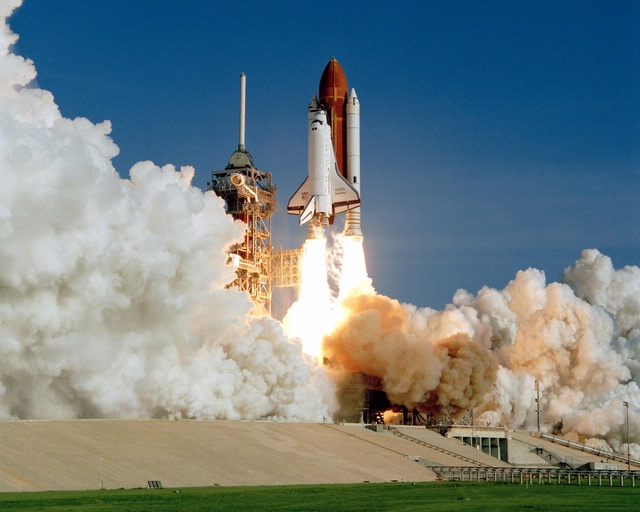
\includegraphics[scale=0.3]{gambar/space-shuttle.jpg}
%  % Keterangan gambar yang diinputkan
%  \caption{Peluncuran pesawat luar angkasa Discovery \citep{DiscoverySpaceShuttle}}
%  % Label referensi dari gambar yang diinputkan
%  \label{fig:SpaceShuttle}
%\end{figure}
%
%Roket luar angkasa merupakan \lipsum[16][1-10]

% Contoh penggunaan referensi dari gambar yang diinputkan
%\emph{Discovery}, Gambar \ref{fig:SpaceShuttle}, merupakan \lipsum[17][1-9]

%\subsection{Hukum Newton}
%
%% Contoh penggunaan referensi dari pustaka
%Newton \citep{Newton1687} pernah merumuskan bahwa \lipsum[19]
%% Contoh penggunaan referensi dari persamaan
%Kemudian menjadi persamaan seperti pada persamaan \ref{eq:FirstNewtonLaw}.
%
%% Contoh pembuatan persamaan
%\begin{equation}
%  % Label referensi dari persamaan yang dibuat
%  \label{eq:FirstNewtonLaw}
%  % Baris kode persamaan yang dibuat
%  \sum \mathbf{F} = 0\; \Leftrightarrow\; \frac{\mathrm{d} \mathbf{v} }{\mathrm{d}t} = 0.
%\end{equation}
%
%\subsection{Anti Gravitasi}
%
%Anti gravitasi merupakan \lipsum[20]
